% coding:utf-8

%FOSAET, a LaTeX-Code for a electrical summary of basic electronics
%Copyright (C) 2013, Daniel Winz, Ervin Mazlagic

%This program is free software; you can redistribute it and/or
%modify it under the terms of the GNU General Public License
%as published by the Free Software Foundation; either version 2
%of the License, or (at your option) any later version.

%This program is distributed in the hope that it will be useful,
%but WITHOUT ANY WARRANTY; without even the implied warranty of
%MERCHANTABILITY or FITNESS FOR A PARTICULAR PURPOSE.  See the
%GNU General Public License for more details.
%----------------------------------------

\section{Logische Verknüpfungen}

\subsection{NOT}
\[ X = \overline{A} \]
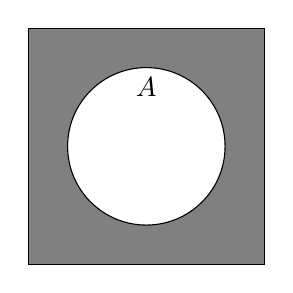
\begin{tikzpicture}
  \fill[gray] (-1.5,-1.5) rectangle (1.5,1.5);
  \draw (-1.5,-1.5) rectangle (1.5,1.5);
  \fill[white] (0,0) circle (1cm);
  \draw (0,0) circle (1cm);
  \draw (0,0.75) node {$A$};
\end{tikzpicture}
\begin{table}[h!]
\[ \begin{array}{c|c}
A&X\\
\hline
0&1\\
1&0
\end{array} \]
\end{table}

\subsection{OR}
\[ X = A \lor B \]
\begin{venndiagram2sets}
  \fillA \fillB
\end{venndiagram2sets}
\begin{table}[h!]
\[ \begin{array}{cc|c}
A&B&X\\
\hline
0&0&0\\
0&1&1\\
1&0&1\\
0&1&1\\
\end{array} \]
\end{table}

\subsection{NOR}
\[ X = \overline{A \lor B} \]
\begin{venndiagram2sets}
  \fillNotAorB
\end{venndiagram2sets}
\begin{table}[h!]
\[ \begin{array}{cc|c}
A&B&X\\
\hline
0&0&1\\
0&1&0\\
1&0&0\\
0&1&0\\
\end{array} \]
\end{table}

\subsection{AND}
\[ X = A \land B \]
\begin{venndiagram2sets}
  \fillACapB
\end{venndiagram2sets}
\begin{table}[h!]
\[ \begin{array}{cc|c}
A&B&X\\
\hline
0&0&0\\
0&1&0\\
1&0&0\\
0&1&1\\
\end{array} \]
\end{table}

\subsection{NAND}
\[ X = \overline{A \land B} \]
\begin{venndiagram2sets}
  \fillNotAorB \fillOnlyA \fillOnlyB
\end{venndiagram2sets}
\begin{table}[h!]
\[ \begin{array}{cc|c}
A&B&X\\
\hline
0&0&1\\
0&1&1\\
1&0&1\\
0&1&0\\
\end{array} \]
\end{table}

\subsection{XOR}
\[ X = A \oplus B \]
\begin{venndiagram2sets}
  \fillOnlyA \fillOnlyB
\end{venndiagram2sets}
\begin{table}[h!]
\[ \begin{array}{cc|c}
A&B&X\\
\hline
0&0&0\\
0&1&1\\
1&0&1\\
0&1&0\\
\end{array} \]
\end{table}

\subsection{XNOR}
\[ X = \overline{A \oplus B} \]
\begin{venndiagram2sets}
  \fillNotAorB \fillACapB
\end{venndiagram2sets}
\begin{table}[h!]
\[ \begin{array}{cc|c}
A&B&X\\
\hline
0&0&1\\
0&1&0\\
1&0&0\\
0&1&1\\
\end{array} \]
\end{table}
